\documentclass{article}
\usepackage{amsmath}
\usepackage{geometry}
\usepackage{tikz}
\usepackage{float}
\usepackage{graphics}
\input{config}

\tikzset{every picture/.style={line width=0.75pt}} %set default line width to 0.75pt        

\begin{document}
\maketitle
\thispagestyle{empty}
\newpage 
\begin{homeworkProblem}[1] 

    Sea $U$ un abierto acotado de $\mathbb{R}^n$ tal que su borde $\partial U=\overline{U}\setminus U$ es de clase $C^1.$ Muestre:
    \begin{itemize}
        \item [i)] \textbf{Formula de integración por partes:} Sean $i=1,\dots,n$ fijo, $u,v\in C^1(\overline{U}).$ Entonces
        $$\int_U(\partial_{x_i}u)v\,dx=\int_{\partial U}(uv)\eta_i\,dS-\int_Uu(\partial_{x_i}v)\,dx,$$
        donde $\eta_i$ es la $i-$ésima componente del vector normal a $\partial U.$
        \begin{solucion}
            Sea $F\in C^1(\overline{U};\mathbb{R}^n)$ un campo vectorial tal que $F=(F_1,\dots,F_n)$, donde $F_i=uv$ para $i=1,\dots,n$ fijo y $F_j=0$ para $j\neq i$, como $F$ cumple las condiciones podemos aplicar el teorema de la divergencia que nos dice que:
            $$\int_Udiv(F)\,dx=\int_{\partial U}F\cdot\eta\,dS.$$ 
            Como tenemos que $F=(0,\dots,uv,\dots,0)$ y $\eta=(\eta_1,\dots,\eta_i,\dots,\eta_n)$, luego
            \begin{align*}
                F\cdot\eta&=(uv)\eta_i,\\
                div(F)&=\partial_{x_i}(uv)=(\partial_{x_i}u)v+u(\partial_{x_i}v).
            \end{align*}
            Así reemplazando en la formula que nos da el teorema de la divergencia, tenemos que:
            $$\int_U(\partial_{x_i}u)v+u(\partial_{x_i}v)\,dx=\int_{\partial U}(uv)\eta_i\,dS.$$
            Luego, por la linealidad de la integral podemos separar y despejar, obteniendo así la formula de integración por partes
            $$\int_U(\partial_{x_i}u)v\,dx=\int_{\partial U}(uv)\eta_i\,dS-\int_Uu(\partial_{x_i}v)\,dx.$$
            \qed
        \end{solucion}
        \item [ii)]\textbf{Formula de Green I:} $\int_U\Delta u\,dx=\int_{\partial U}\nabla u\cdot\eta\,dS,$ donde $\eta$ es el vector normal a la superficie $\partial U.$
        \begin{solucion}
            Por definición del Laplaciano tenemos que:
            \begin{align*}
                \int_U\Delta u\,dx&=\int_U\left(\sum_{i=1}^n\partial^2_{x_i}u\right)\,dx\\
                &=\sum_{i=1}^n\int_U\partial^2_{x_i}u\,dx.
            \end{align*}
            Esto lo podemos hacer por la linealidad de la integral, ya que es una suma finita. Ahora note que a $\int_U\partial^2_{x_i}u\,dx$ podemos aplicar la formula de integración por partes obtenida en $i).$ Consideremos la siguiente reescritura de la integral para verla de forma más clara:
            $$\int_U(\partial_{x_i}(\partial_{x_i}u))\cdot1\,dx.$$
            Es decir, nuestro $v=1$ y la otra función es $\partial_{x_i}u$. Por la formula de integración por partes:
            $$\int_U\partial^2_{x_i}u\,dx=\int_{\partial U}(\partial_{x_i}u\cdot1)\eta_i\,dS-\int_U\partial_{x_i}u(\partial_{x_i}1)\,dx.$$
            Pero como $\partial_{x_i}1=0$ para todo $i=1,\dots,n,$ obtenemos que
            $$\int_U\partial^2_{x_i}u\,dx=\int_{\partial U}(\partial_{x_i}u)\eta_i\,dS.$$
            Reemplazando este resultado y nuevamente por linealidad, de lo cual tenemos
            \begin{align*}
                \sum_{i=1}^n\int_U\partial^2_{x_i}u\,dx&=\sum_{i=1}^n\int_{\partial U}(\partial_{x_i}u)\eta_i\,dS\\
                &=\int_{\partial U}\left(\sum_{i=1}^n(\partial_{x_i}u)\eta_i\right)\,dS.
            \end{align*}
            Note que,
            $$\sum_{i=1}^n(\partial_{x_i}u)\eta_i=(\partial_{x_1}u,\dots,\partial_{x_n}u)\cdot(\eta_1,\dots,\eta_n)=\nabla u\cdot\eta.$$
            Y si reemplazamos, da como resultado:
            $$\int_{\partial U}\left(\sum_{i=1}^n(\partial_{x_i}u)\eta_i\right)\,dS=\int_{\partial U}\nabla u\cdot\eta\,dS$$
            De esta forma hemos mostrado que:
            $$\int_U\Delta u\,dx=\int_{\partial U}\nabla u\cdot\eta\,dS.$$
            \qed 
        \end{solucion}
        \item [iii)] \textbf{Formula de Green II: }$\int_U\nabla u\cdot\nabla v\,dx=-\int_U u\Delta v\,dx+\int_{\partial U}u(\nabla v\cdot\eta)\,dS.$
        \begin{solucion}
            Note que
            $$\nabla u\cdot\nabla v=(\partial_{x_1}u,\dots,\partial_{x_n}u)\cdot(\partial_{x_1}v,\dots,\partial_{x_n}v)=\sum_{i=1}^n(\partial_{x_i}u)(\partial_{x_i}v).$$
            Reemplazando y por la linealidad, obtenemos
            \begin{align*}
                \int_U\nabla u\cdot\nabla v\,dx&=\int_U\sum_{i=1}^n(\partial_{x_i}u)(\partial_{x_i}v)\,dx\\
                &=\sum_{i=1}^n\int_U(\partial_{x_i}u)(\partial_{x_i}v)\,dx.
            \end{align*}
            Ahora, apliquemos la formula de integración por partes a la integral dentro de la sumatoria
            $$\int_U(\partial_{x_i}u)(\partial_{x_i}v)\,dx=\int_{\partial U}(u\partial_{x_i}v)\eta_i\,dS-\int_Uu(\partial_{x_i}^2v)\,dx.$$
            Reemplazando en la sumatoria, reordenando los términos y usando nuevamente la linealidad, tenemos:
            \begin{align*}
             \sum_{i=1}^n\int_U(\partial_{x_i}u)(\partial_{x_i}v)\,dx&=\sum_{i=1}^n\left(\int_{\partial U}(u\partial_{x_i}v)\eta_i\,dS-\int_Uu(\partial_{x_i}^2v)\,dx\right)\\
             &=\sum_{i=1}^n\left(-\int_Uu(\partial_{x_i}^2v)\,dx\right)+\sum_{i=1}^n\left(\int_{\partial U}(u\partial_{x_i}v)\eta_i\,dS\right)\\
             &=-\int_U\left(\sum_{i=1}^nu(\partial_{x_i}^2v)\right)\,dx+\int_{\partial U}\left(\sum_{i=1}^n(u\partial_{x_i}v)\eta_i\right)\,dS.
            \end{align*}
            Note que cada sumatoria la podemos reescribir como:
            \begin{align*}
              \sum_{i=1}^nu(\partial_{x_i}^2v)&=u\sum_{i=1}^n(\partial_{x_i}^2v)=u\Delta v,\\
              \sum_{i=1}^n(u\partial_{x_i}v)\eta_i&=u\sum_{i=1}^n(\partial_{x_i}v)\eta_i=u(\nabla v\cdot\eta).
            \end{align*}
            Luego, reemplazando en la expresión obtenida:
            $$-\int_U\left(\sum_{i=1}^nu(\partial_{x_i}^2v)\right)\,dx+\int_{\partial U}\left(\sum_{i=1}^n(u\partial_{x_i}v)\eta_i\right)\,dS=-\int_Uu\Delta v\,dx+\int_{\partial U}u(\nabla v\cdot\eta)\,dS.$$
            Así hemos mostrado que:
            $$\int_U\nabla u\cdot\nabla v\,dx=-\int_U u\Delta v\,dx+\int_{\partial U}u(\nabla v\cdot\eta)\,dS.$$
            \qed
        \end{solucion}
        \item [iv)] \textbf{Formula de Green III: }$\int_{U}(u\Delta v-v\Delta u)\,dx=\int_{\partial U}\left(u(\nabla v\cdot\eta)-v(\nabla u\cdot\eta)\right)\,dS.$
        \begin{solucion}
            Por la formula de Green II tenemos que:
            $$\int_U\nabla u\cdot\nabla v\,dx=-\int_U u\Delta v\,dx+\int_{\partial U}u(\nabla v\cdot\eta)\,dS.$$
            Si consideramos $\int_{U}\nabla v\cdot\nabla u\,dx$, podemos aplicar nuevamente la formula de Green II
            $$\int_U\nabla v\cdot\nabla u\,dx=-\int_U v\Delta u\,dx+\int_{\partial U}v(\nabla u\cdot\eta)\,dS.$$ 
            Si a la primera expresión le restamos la segunda obtenemos:\
            \begin{multline*}
                \int_U\nabla u\cdot\nabla v\,dx-\int_U\nabla v\cdot\nabla u\,dx=-\int_U u\Delta v\,dx+\int_{\partial U}u(\nabla v\cdot\eta)\,dS
                \\+\int_U v\Delta u\,dx-\int_{\partial U}v(\nabla u\cdot\eta)\,dS
            \end{multline*}
            Luego por linealidad
            $$\int_U(\nabla u\cdot\nabla v-\nabla v\cdot\nabla u)\,dx=-\int_{U}(u\Delta v-v\Delta u)\,dx+\int_{\partial U}\left(u(\nabla v\cdot\eta)-v(\nabla u\cdot\eta)\right)\,dS.$$
            Recordemos que el producto punto es conmutativo, por lo tanto $\nabla u\cdot\nabla v-\nabla v\cdot\nabla u=0$. Es decir, que la expresión anterior es en realidad la siguiente:
            $$0=-\int_{U}(u\Delta v-v\Delta u)\,dx+\int_{\partial U}\left(u(\nabla v\cdot\eta)-v(\nabla u\cdot\eta)\right)\,dS.$$
            De esta manera, simplemente despejando hemos demostrado
            $$\int_{U}(u\Delta v-v\Delta u)\,dx=\int_{\partial U}\left(u(\nabla v\cdot\eta)-v(\nabla u\cdot\eta)\right)\,dS.$$
            \qed
        \end{solucion}
    \end{itemize}
\end{homeworkProblem}
\newpage
\begin{homeworkProblem}[3]
    Muestre que la ecuación de Laplace $\Delta u=0$ es invariante por rotaciones. Mas precisamente, muestre que si $O$ es una matriz ortogonal de tamaño $n\times n$ y definimos $v(x)=u(Ox),$ entonces $\Delta v=0.$
    \begin{solucion}
        Para no tener confusiones con la notación definimos $v(x)=u(y)$ donde $y=Ox$. Mas explícitamente si $O=(o_{ij})_{1\leq i,j\leq n}$ y $x=(x_1,\dots,x_n),$ tenemos que si $y=(y_1,\dots,y_n)$ entonces $y_l=\sum_{m=1}^no_{lm}x_m,$ con $1\leq l\leq n.$ \\
        Note que cada uno de los $y_l$ depende de todos los $x_i$, luego la primera derivada de $v$ respecto a $x_i$ por regla de la cadena es:
        $$\partial_{x_i}v=\sum_{l=1}^n(\partial_{y_l}u)(\partial_{x_i}y_l)=\sum_{l=1}^no_{li}\partial_{y_l}u.$$
        Para la segunda derivada, por la regla de la cadena tenemos 
        $$\partial^2_{x_i}v=\sum_{l=1}^no_{li}\sum_{k=1}^n(\partial_{y_k}\partial_{y_l}u)(\partial_{x_i}y_k)=\sum_{l=1}^n\sum_{k=1}^no_{li}o_{ki}(\partial_{y_k}\partial_{y_l}u).$$
        Luego por la definición del Laplaciano
        $$\Delta v=\sum_{i=1}^n\partial^2_{x_i}v=\sum_{i=1}^n\sum_{l=1}^n\sum_{k=1}^no_{li}o_{ki}(\partial_{y_k}\partial_{y_l}u).$$
        Antes de continuar con esta sumatoria, recordemos que por hipótesis nuestra matriz $O$ es ortogonal, eso quiere decir que $O\cdot O^T=I.$ Tengamos en cuenta que la entrada de la fila $i$ y columna $j$ de la matriz $O\cdot O^T$ esta dada por:
        $$(O\cdot O^T)_{ij}=\sum_{k=1}^no_{ik}o_{jk}.$$
        Pero como la matriz $O\cdot O^T$ es igual a la matriz identidad de tamaño $n\times n$ tenemos que:
        $$\sum_{k=1}^no_{ik}o_{jk}=\begin{cases}
         1, & i=j,\\
         0, & i\neq j.
        \end{cases}$$
        Volviendo a la sumatoria encontrada previamente, por ser sumas finitas podemos reorganizarla a conveniencia, en particular estudiémosla en el siguiente orden
        $$\Delta v=\sum_{l=1}^n\sum_{k=1}^n\sum_{i=1}^no_{li}o_{ki}(\partial_{y_k}\partial_{y_l}u).$$
        Note que la sumatoria interior es particularmente la entrada $(l,k)$ de la matriz $O\cdot O^T$ multiplicada por las derivadas parciales. Luego las otras dos sumatorias van sobre todas las filas $l$ y columnas $k$ de esta matriz. Pero, nosotros sabemos que esta matriz es la identidad, por lo que solo quedan los términos de la diagonal. Es decir, cuando $l=k$ es cuando no se harán $0$, y por hipótesis $\Delta u=0$, así:
        \begin{align*}
            \Delta v&=\sum_{l=1}^n\sum_{k=1}^n\sum_{i=1}^no_{li}o_{ki}(\partial_{y_k}\partial_{y_l}u)\\
            &=\sum_{i=1}^no_{1i}o_{1i}(\partial_{y_1}\partial_{y_1}u)+\cdots+\sum_{i=1}^no_{ni}o_{ni}(\partial_{y_n}\partial_{y_n}u)\\
            &=\partial_{y_1}^2u+\cdots+\partial_{y_n}^2u\\
            &=\Delta u\\&=0.
        \end{align*}
        De esta manera, hemos concluido que $\Delta v=0.$ Es decir que la ecuación de Laplace es invariante por rotaciones.
        \qed
    \end{solucion}
\end{homeworkProblem}
\newpage
\begin{homeworkProblem}[6]
   En $\mathbb{R}^2$, encuentre la función de Green para el primer cuadrante $U=\{(x,y):x>0,y>0\}.$ Verifique su respuesta.
   \begin{solucion}
   Seguiremos una idea similar a la del semiespacio $\mathbb{R}^n_+.$ Sea $x=(x_1,x_2)\in U$, consideremos las siguientes ``reflexiones'' del punto $x$:
    \begin{center}
        

\tikzset{every picture/.style={line width=0.75pt}} %set default line width to 0.75pt        

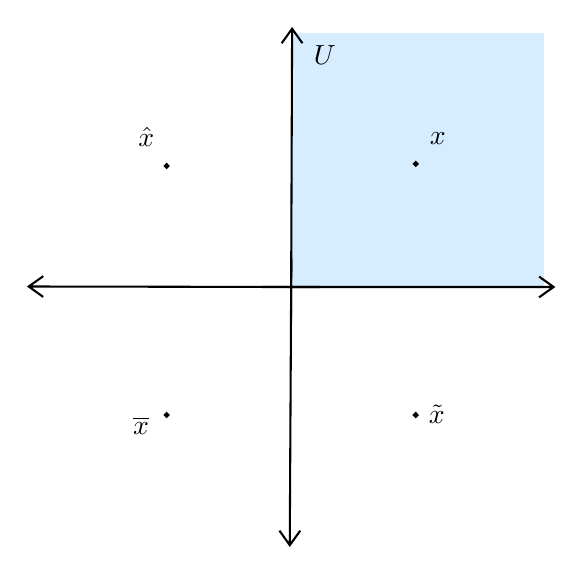
\begin{tikzpicture}[x=0.75pt,y=0.75pt,yscale=-1,xscale=1]
%uncomment if require: \path (0,300); %set diagram left start at 0, and has height of 300

%Flowchart: Process [id:dp5061113551178431] 
\draw  [color={rgb, 255:red, 255; green, 255; blue, 255 }  ,draw opacity=1 ][fill={rgb, 255:red, 214; green, 236; blue, 255 }  ,fill opacity=1 ] (330.11,35.93) -- (452.36,35.93) -- (452.36,158.68) -- (330.11,158.68) -- cycle ;
%Shape: Axis 2D [id:dp10735875164774633] 
\draw  (316.06,158.68) -- (456.55,158.68)(330.56,34.25) -- (330.05,172.5) (449.57,153.68) -- (456.55,158.68) -- (449.53,163.68) (325.54,41.25) -- (330.56,34.25) -- (335.54,41.25)  ;
%Shape: Axis 2D [id:dp2784724280913353] 
\draw  (344.16,158.7) -- (203.66,158.45)(329.43,283.1) -- (330.18,144.85) (210.63,163.47) -- (203.66,158.45) -- (210.69,153.47) (334.47,276.11) -- (329.43,283.1) -- (324.47,276.09)  ;
%Shape: Circle [id:dp07309661543089163] 
\draw  [fill={rgb, 255:red, 0; green, 0; blue, 0 }  ,fill opacity=1 ] (389.25,99.38) .. controls (389.25,98.89) and (389.64,98.5) .. (390.13,98.5) .. controls (390.61,98.5) and (391,98.89) .. (391,99.38) .. controls (391,99.86) and (390.61,100.25) .. (390.13,100.25) .. controls (389.64,100.25) and (389.25,99.86) .. (389.25,99.38) -- cycle ;
%Shape: Circle [id:dp48259078447118964] 
\draw  [fill={rgb, 255:red, 0; green, 0; blue, 0 }  ,fill opacity=1 ] (389.25,220.38) .. controls (389.25,219.89) and (389.64,219.5) .. (390.13,219.5) .. controls (390.61,219.5) and (391,219.89) .. (391,220.38) .. controls (391,220.86) and (390.61,221.25) .. (390.13,221.25) .. controls (389.64,221.25) and (389.25,220.86) .. (389.25,220.38) -- cycle ;
%Shape: Circle [id:dp9234675238862919] 
\draw  [fill={rgb, 255:red, 0; green, 0; blue, 0 }  ,fill opacity=1 ] (269.25,100.38) .. controls (269.25,99.89) and (269.64,99.5) .. (270.13,99.5) .. controls (270.61,99.5) and (271,99.89) .. (271,100.38) .. controls (271,100.86) and (270.61,101.25) .. (270.13,101.25) .. controls (269.64,101.25) and (269.25,100.86) .. (269.25,100.38) -- cycle ;
%Shape: Circle [id:dp900863572025848] 
\draw  [fill={rgb, 255:red, 0; green, 0; blue, 0 }  ,fill opacity=1 ] (269.25,220.38) .. controls (269.25,219.89) and (269.64,219.5) .. (270.13,219.5) .. controls (270.61,219.5) and (271,219.89) .. (271,220.38) .. controls (271,220.86) and (270.61,221.25) .. (270.13,221.25) .. controls (269.64,221.25) and (269.25,220.86) .. (269.25,220.38) -- cycle ;

% Text Node
\draw (395.5,82.9) node [anchor=north west][inner sep=0.75pt]    {$x$};
% Text Node
\draw (252.5,219.9) node [anchor=north west][inner sep=0.75pt]    {$\overline{x}$};
% Text Node
\draw (395,213.9) node [anchor=north west][inner sep=0.75pt]    {$\tilde{x}$};
% Text Node
\draw (255,80.4) node [anchor=north west][inner sep=0.75pt]    {$\hat{x}$};
% Text Node
\draw (339.5,40.9) node [anchor=north west][inner sep=0.75pt]    {$U$};


\end{tikzpicture}
    \end{center}
   Donde $\Tilde{x}=(x_1,-x_2),\,\hat{x}=(-x_1,x_2)$ y $\bar{x}=(-x_1,-x_2)$, entonces nuestro candidato a función correctora será:
   $$\phi^x(y)=\Phi(y-\Tilde{x})+\Phi(y-\hat{x})-\Phi(y-\bar{x})$$
   Verifiquemos si satisface las dos condiciones, la primera que debe de satisfacer es: $\Delta\phi^x=0$ en $U$, entonces sea $y\in U$,
   $$\Delta\phi^x(y)=\Delta\Phi(y-\Tilde{x})+\Delta\Phi(y-\hat{x})-\Delta\Phi(y-\bar{x}).$$
   Luego, como $\Tilde{x},\hat{x},\bar{x}\notin U$ tenemos que no hay singularidades. Por tanto $\Phi$ es la solución fundamental, lo cual implica $\Delta\Phi(y-\Tilde{x})=\Delta\Phi(y-\hat{x})=\Delta\Phi(y-\bar{x})=0,$ concluimos que:
   $$\Delta\phi^x(y)=0.$$
   La segunda condición nos dice: $\phi^x(y)=\Phi(y-x)$ en $\partial U.$ Notemos primero que\\ $\partial U=\{(x,y):x=0,y>0\}\cup\{(x,y):x>0,y=0\}\cup\{(0,0)\}$.\\ Para mostrar esta condición consideremos los tres casos posibles:
   \begin{itemize}
       \item \textbf{Caso 1: }Sea $y=(0,y_2)$ con $y_2>0$, tenemos que:
       \begin{align*}
           \phi^x(y)&=\phi^x((0,y_2))\\
           &=\Phi((0,y_2)-(x_1,-x_2))+\Phi((0,y_2)-(-x_1,x_2))-\Phi((0,y_2)-(-x_1,-x_2))\\
           &=\Phi((-x_1,y_2+x_2))+\Phi((x_1,y_2-x_2))-\Phi((x_1,y_2+x_2)).
       \end{align*}
        Note que $|(-x_1,y_2+x_2)|=|(x_1,y_2+x_2)|$ y $|(x_1,y_2-x_2)|=|(-x_1,y_2-x_2)|$. Luego como $\Phi$ es radial obtenemos que $\Phi((-x_1,y_2+x_2))=\Phi((x_1,y_2+x_2))$ y $\Phi((x_1,y_2-x_2))=\Phi((-x_1,y_2-x_2))$, así podemos concluir:
       \begin{align*}
        \phi^x(y)&=\Phi((-x_1,y_2+x_2))+\Phi((x_1,y_2-x_2))-\Phi((x_1,y_2+x_2))\\
        &=\Phi((-x_1,y_2-x_2))\\
        &=\Phi((0,y_2)-(x_1,x_2))\\
        &=\Phi(y-x)
       \end{align*}
       \item \textbf{Caso 2: }Sea $y=(y_1,0)$ con $y_1>0$, tenemos que:
       \begin{align*}
           \phi^x(y)&=\phi^x((y_1,0))\\
           &=\Phi((y_1,0)-(x_1,-x_2))+\Phi((y_1,0)-(-x_1,x_2))-\Phi((y_1,0)-(-x_1,-x_2))\\
           &=\Phi((y_1-x_1,x_2))+\Phi((y_1+x_1,-x_2))-\Phi((y_1+x_1,x_2)).
       \end{align*}
       Note que $|(y_1+x_1,-x_2)|=|(y_1+x_1,x_2)|$ y $|(y_1-x_1,x_2)|=|(y_1-x_1,-x_2)|$. Luego como $\Phi$ es radial obtenemos que $\Phi((y_1+x_1,-x_2))=\Phi((y_1+x_1,x_2))$ y $\Phi((y_1-x_1,x_2))=\Phi((y_1-x_1,-x_2))$, así podemos concluir:
       \begin{align*}
        \phi^x(y)&=\Phi((y_1-x_1,x_2))+\Phi((y_1+x_1,-x_2))-\Phi((y_1+x_1,x_2))\\
        &=\Phi((y_1-x_1,-x_2))\\
        &=\Phi((y_1,0)-(x_1,x_2))\\
        &=\Phi(y-x)
       \end{align*}
       \item \textbf{Caso 3: }Sea $y=(0,0),$ tenemos que:
       \begin{align*}
           \phi^x(y)&=\phi^x((0,0))\\
           &=\Phi((0,0)-(x_1,-x_2))+\Phi((0,0)-(-x_1,x_2))-\Phi((0,0)-(-x_1,-x_2))\\
           &=\Phi((-x_1,x_2))+\Phi((x_1,-x_2))-\Phi((x_1,x_2)).
       \end{align*}
       Note que $|(-x_1,x_2)|=|(x_1,-x_2)|=|(x_1,x_2)|=|(-x_1,-x_2)|,$ luego como $\Phi$ es radial obtenemos que $\Phi((-x_1,-x_2))=\Phi((x_1,-x_2))=\Phi((-x_1,x_2))=\Phi((x_1,x_2)),$ así podemos concluir: 
       \begin{align*}
        \phi^x(y)&=\Phi((-x_1,x_2))+\Phi((x_1,-x_2))-\Phi((x_1,x_2))\\
        &=\Phi((-x_1,-x_2))+\Phi((-x_1,-x_2))-\Phi((-x_1,-x_2))\\
        &=\Phi((-x_1,-x_2))\\
        &=\Phi((0,0)-(x_1,x_2))\\
        &=\Phi(y-x).
       \end{align*} 
   \end{itemize}
   De esta forma, concluimos que dado $y\in \partial U$, $\phi^x(y)=\Phi(y-x).$ Como nuestra propuesta de función correctora satisface las dos condiciones, podemos decir que la función de Green para el primer cuadrante es:
   $$G(x,y):=\Phi(y-x)-\phi^x(y)=\Phi(y-x)-\Phi(y-\Tilde{x})-\Phi(y-\hat{x})+\Phi(y-\bar{x}).$$
   \qed
   \end{solucion}
\end{homeworkProblem}
\newpage
\begin{homeworkProblem}[8]
    Sean $U$ un abierto acotado con borde suave y $u\in C^2(\overline{U})$ la solución del problema:
    $$\begin{cases}
        -\Delta u=f& \text{en }U,\\
        \phantom{-\Delta}u=g & \text{en }\partial U,
    \end{cases}$$
    donde $f$ y $g$ son funciones continuas. Definimos el conjunto $\mathcal{A}=\{w\in C^2(\overline{U}):w=g\text{ en }\partial U\}$ y el funcional de energía
    $$E[w]=\int_U\left(\dfrac{1}{2}|\nabla w|^2-wf\right)\,dx.$$
    Muestre que 
    $$E[u]=\min_{w\in\mathcal{A}}E[w].$$
    Es decir, soluciones de la EDP minimizan el funcional de energía $E[\cdot].$
\end{homeworkProblem}
\begin{solucion}
    Sea $w\in\mathcal{A},$ como $u$ es solución de la EDP, tenemos que $-\Delta u=f$, por tanto $\Delta u+f=0$ así,
    $$\int_U(\Delta u+f)(u-w)\,dx=0.$$
    Estudiemos la integral del lado izquierdo. Si realizamos el producto y aplicamos la linealidad, obtenemos que
    $$\int_U(u-w)(\Delta u+f)\,dx=\int_Uu\Delta u\,dx+\int_U uf\,dx-\int_Uw\Delta u-\int_U wf\,dx.$$
    Si consideramos la \textbf{Formula de Green II} usando las funciones $u$ y $w$ tenemos que:
    \begin{align*}
      \int_U\nabla u\cdot\nabla u\,dx&=-\int_U u\Delta u\,dx+\int_{\partial U}u(\nabla u\cdot\eta)\,dS,\\
      \int_U\nabla w\cdot\nabla u\,dx&=-\int_U w\Delta u\,dx+\int_{\partial U}w(\nabla u\cdot\eta)\,dS.
    \end{align*}
    Note que en estas aparecen dos términos de la integral que estamos estudiando. Si los despejamos nos da que:
    \begin{align*}
     \int_U u\Delta u\,dx&=\int_{\partial U}u(\nabla u\cdot\eta)\,dS-\int_U\nabla u\cdot\nabla u\,dx,\\
     -\int_U w\Delta u\,dx&=\int_U\nabla w\cdot\nabla u\,dx-\int_{\partial U}w(\nabla u\cdot\eta)\,dS.
    \end{align*}
    Como $u=g$ en $\partial U$, ya que $u$ es solución de la EDP y $w=g$ en $\partial U$ dado que $w\in\mathcal{A}$. Además, $\nabla u\cdot \nabla u=|\nabla u|^2,$ reemplazando obtenemos
    \begin{align*}
      \int_U u\Delta u\,dx&=\int_{\partial U}g(\nabla u\cdot\eta)\,dS-\int_U|\nabla u|^2\,dx,\\
     -\int_U w\Delta u\,dx&=\int_U\nabla w\cdot\nabla u\,dx-\int_{\partial U}g(\nabla u\cdot\eta)\,dS,  
    \end{align*}
    y sumando ambas expresiones tenemos
    $$\int_U u\Delta u\,dx-\int_U w\Delta u\,dx=\int_U\nabla w\cdot\nabla u\,dx-\int_U|\nabla u|^2\,dx.$$
    Podemos reemplazar lo obtenido en nuestra expresión original:
    $$\int_Uu\Delta u\,dx+\int_U uf\,dx-\int_Uw\Delta u-\int_U wf\,dx=\int_U\nabla w\cdot\nabla u\,dx-\int_U|\nabla u|^2\,dx+\int_U uf\,dx-\int_U wf\,dx$$
    Ahora por las desigualdades de Cauchy-Schwarz y Young respectivamente,
    \begin{align*}
        \int_U\nabla w\cdot\nabla u\,dx&\leq\int_U|\nabla w\cdot\nabla u|\,dx\\
        &\leq\int_U|\nabla w|\cdot|\nabla u|\,dx\\
        &\leq\int_U\dfrac{1}{2}|\nabla w|^2+\dfrac{1}{2}|\nabla u|^2\,dx\\
        &=\int_U\dfrac{1}{2}|\nabla w|^2\,dx+\int_U\dfrac{1}{2}|\nabla u|^2\,dx.
    \end{align*}
    Usando esta desigualdad y recordando que nuestra integral original es igual a 0,
    $$0\leq\int_U\dfrac{1}{2}|\nabla w|^2\,dx+\int_U\dfrac{1}{2}|\nabla u|^2\,dx-\int_U|\nabla u|^2\,dx+\int_U uf\,dx-\int_U wf\,dx.$$
    Reorganizando la expresión,
    $$\int_U\left(\dfrac{1}{2}|\nabla u|^2-uf\right)\,dx\leq\int_U\left(\dfrac{1}{2}|\nabla w|^2-wf\right)\,dx.$$
    Note que esta es la definición del funcional de energía, por lo que es equivalente escribir:
    $$E[u]\leq E[w].$$
    Por otro lado, $u\in\mathcal{A}$ por lo que $E[u]\in\{E[w]:w\in\mathcal{A}\}\neq\varnothing$ y como $E[u]\leq E[w]$ para todo $w\in\mathcal{A}$, ya que lo consideramos arbitrario al principio, podemos concluir:
    $$E[u]=\min_{w\in\mathcal{A}}E[w].$$
    \qed
\end{solucion}
%%%%%%%%%%%%%%%%%%%%%%%%%%%%%%%%%%%%%%%%%%%%%%%%%%%%%%%
\end{document}